% ============================================================
%  深圳大学实验报告模板（SZU Experiment Report Template）
% This template can be modified according to the specific requirements of your experiment or project.
% Produced by: Chao Fan and Kewei Ou, AI School of SZU
% ============================================================

\documentclass[a4paper,12pt]{article}

% ----------------------------
% 中文与字体支持
% ----------------------------
\usepackage{fontspec}    % 字体支持
\usepackage{xeCJK}       % 中文字体支持
\setCJKmainfont{Noto Serif CJK SC} % 设置中文字体（Overleaf自带Noto字体）

% ----------------------------
% 页面设置与常用宏包
% ----------------------------
\usepackage{geometry}    % 页面边距控制
\geometry{left=1in, right=1in, top=1in, bottom=1in}

\usepackage{longtable}   % 支持长表格
\usepackage{graphicx}    % 插入图片
\usepackage{fancyhdr}    % 页眉页脚控制
\usepackage{tikz}        % 绘制框线等图形
\usetikzlibrary{calc}    % 坐标计算
\usepackage{verbatim}    % 显示代码块
\usepackage{float}       % 控制图片浮动位置（[H]参数）
\usepackage{hyperref}    % 超文本链接

% ----------------------------
% 页眉页脚设置
% ----------------------------
\pagestyle{fancy}
\fancyhf{} % 清空默认页眉页脚
\fancyhead[L]{深圳大学实验报告} % 左侧页眉文字
\fancyhead[C]{} % 中间空
\fancyhead[R]{} % 右侧空

% ============================================================
%                      文档开始
% ============================================================

\begin{document}

% ============================================================
% 封面页
% ============================================================
\begin{titlepage}
    \centering
    \vspace*{2cm}
    \Huge{\textbf{深 \ 圳 \ 大 \ 学 \ 实 \ 验  \ 报 \ 告}}\\[1.5cm]
    
    \Large{课程名称：\underline{\makebox[8cm][c]{Python程序设计}}}\\[0.5cm]
    \Large{项目名称：\underline{\makebox[8cm][c]{《外星人入侵》小游戏}}}\\[0.5cm]
    \Large{学 \quad \quad 院：\underline{\makebox[8cm][c]{人工智能学院}}}\\[0.5cm]
    \Large{专 \quad \quad 业：\underline{\makebox[8cm][c]{计算机科学与技术（IEEE）}}}\\[0.5cm]
    \Large{指导教师：\underline{\makebox[8cm][c]{樊超、舒婷}}}\\[0.5cm]
 \Large
报告人：\underline{\makebox[3.55cm][c]{朱明钊}}%
\hspace{0.5cm}%
学号：\underline{\makebox[2.8cm][c]{2024341011}}\\[0.5cm]
    \Large{实验时间：\underline{\makebox[8cm][c]{2025年11月12日-11月25日}}}\\[0.5cm]
    \Large{提交时间：\underline{\makebox[8cm][c]{2025年11月25日}}}\\[1.5cm]

    \vfill
    \Large{教务处制}
\end{titlepage}

\newpage

% ============================================================
% 正文部分
% ============================================================
% Experiment Objectives


\section{实验目的}

%Describe the goal of the experiment, including what you aim to achieve (e.g., testing an algorithm, solving a problem, or exploring a concept).

{开发一款可交互的 2D 射击游戏《外星人入侵》，巩固 Python 面向对象、事件驱动与碰撞检测知识；同时练习使用 XeLaTeX 撰写技术报告。}


% Experiment Process
\section{实验概述}
%briefly outline the approach and methods used in the experiment.
\begin{enumerate}
    \item[Spot 1]: 采用 \texttt{pygame} 引擎，60 FPS 主循环驱动;
    \item[Spot 2]: 基本类与功能：\texttt{Alien}, \texttt{Bullet}, \texttt{Explosion}, \texttt{GameStats}, \texttt{Scoreboard} ;
    \item[Spot 3]: \textcolor{red} {拓展功能}： 存储分数 + 连击系统 + 爆炸特效：命中后实时更新 combo 并播放爆炸特效与音效;
\end{enumerate}

% Implementation Details
\section{关键实现}
%Provide a high-level overview of the key parts of your code.

Figure ~\ref{fig:module}给出主要类及其职责划分:
\begin{figure}[H]
  \centering
  \includegraphics[width=0.95\linewidth]{module.png}
  \caption{模块划分与类职责}
  \label{fig:module}
\end{figure}

\begin{enumerate}
\item 基本类：
    \item[AlienInvasion]: 管理游戏资源和行为的类（最核心）;
    \item[Alien]: 表示单个外星人的类;
    \item[Bullet]: 管理飞船所发射的子弹的类;
    \item[Button]: 为游戏创建按钮的类
    \item[GameStats]: 跟踪游戏统计信息的类
    \item[ScoreBoard]: 显示得分信息的类
    \item[Settings]:存储游戏《 Alien Invasion 》中所有设置的类
    \item[Ship]: 管理飞船的类
\item 附加功能：
    \item[存储分数]:集成在GameStats与ScoreBoard中 ,可将历史最高分数记录在本地
    \item[连击系统]:集成在Bullet类中，短时间内连击次数越多，得分加成越大
    \item[爆炸特效]:调用pygame的音效库，让游戏更有趣。外星人被击中后，会爆炸
\end{enumerate}

\subsection*{时序图梳理}

Figure ~\ref{fig:sequence} 展示了一次“子弹击中外星人”的完整控制流。
每帧60~FPS循环内，各对象按自上而下顺序完成一次消息传递：

\begin{figure}[H]
  \centering
  \includegraphics[width=0.95\linewidth]{sequence.png}
  \caption{击中→更新连击→爆炸→音效→刷新UI的时序}
  \label{fig:sequence}
\end{figure}

\begin{enumerate}
  \item \textbf{AlienInvasion} 主循环调用 \texttt{\_update\_bullets()}；
  \item \textbf{Bullet} 与 \textbf{Alien} 碰撞检测，返回被击中外星人列表；
  \item \textbf{GameStats} 先 \texttt{update\_combo()} 累加连击，再将分数与得分系数乘算，更新得分；
  \item 为每个被击中外星人新建爆炸特效；
  \item \textbf{SoundManager} 同步 \texttt{play\_explosion()} 播放音效；
  \item \textbf{Scoreboard} 调用 \texttt{prep\_score()} 与 \texttt{prep\_combo()}
        重绘得分板；
  \item 最后 \textbf{AlienInvasion} 执行 \texttt{\_update\_screen()} 完成画面刷新。
\end{enumerate}

\textcolor{red}{整个序列在一帧内结束，保证视觉、数据、音效实时同步}



\section{实验结果}

%Present the output generated by your program. 
%Include any test cases, screenshots, or tables of results.
Figure ~\ref{fig:text} 展现了实际的游戏画面，\textcolor{red}{基本游戏功能已较为完善}
\begin{figure}
    \centering
    \includegraphics[width=0.95\linewidth]{text.png}
    \caption{游戏实机演示画面}
    \label{fig:text}
\end{figure}

\section{讨论与改进}

%Analyze the performance of your program. 
%Discuss any errors, inefficiencies, or areas for improvement. 
通过本次实验，将课堂所学的面向对象、事件驱动与碰撞检测知识整合为可玩的完整游戏，我深刻体会到：

\begin{itemize}
  \item 模块化设计能显著降低调试难度，一人维护 11 个类依然可快速定位缺陷；
  \item 先大致想好所需功能，然后就动手开写代码。先行动起来，日后可逐渐重构代码
  \item 连击+爆炸+音效的即时反馈是提升玩家沉浸感的关键，数据与表现需在同一帧内完成。
\end{itemize}

不足之处

\begin{itemize}
    \item 代码经验不足，实验耗时较长
    \item 尚不能熟练使用github与 \LaTeX 等工具辅助开发、汇报
    \item 拓展功能的实现，借助了AI辅助开发
\end{itemize}

\href {https://github.com/coool-day/Python-project} {Github项目地址}

\newpage

% ============================================================
% 批阅与成绩评定页
% ============================================================

% 绘制正文外框（包含批阅区域）
\begin{tikzpicture}[remember picture, overlay]
  \draw[thick] 
    ($(current page.north west)+(2cm,-3cm)$) 
    rectangle 
    ($(current page.south east)+(-2cm,2.5cm)$);
\end{tikzpicture}

\vspace{1cm}

% 批阅区
\noindent \textbf{指导教师批阅意见：}
\vspace{5cm}
\hfill

\vspace{1cm}

\noindent \textbf{成绩评定：}
\vspace{2cm}
\hfill

\vspace{1cm}

\noindent \textbf{指导教师签字：}
\vspace{2cm}
\hfill

\vspace{1cm}

% 备注部分
\noindent \textbf{备注：}
\begin{itemize}
    \item 报告内的项目或内容设置，可根据实际情况加以调整和补充。
    \item 教师批改学生实验报告时间应在学生提交实验报告时间后 10 日内。
\end{itemize}

% ============================================================
%                      文档结束
% ============================================================

\end{document}